\documentclass[12pt,letterpaper]{report}

\marginparsep 0pt
\textwidth 6in
\topmargin 0pt
\headsep .5in
\textheight 9.2in
\voffset = 0pt
\hoffset = 0pt
\marginparwidth = 0pt \oddsidemargin = 0pt \sloppy

%Dimensiones de la página
\usepackage[left=2.5cm,top=3cm,right=2.5cm,bottom=2.5cm]{geometry}
%Sangría
\setlength{\parindent}{1cm}

%Numeracion
\pagenumbering{arabic}

\usepackage[utf8]{inputenc}
\usepackage[spanish]{babel}
\usepackage{graphicx}
\usepackage{graphics}
\usepackage[dvips]{epsfig}
\usepackage[dvips]{graphicx}
\usepackage{rotating}
\usepackage{multirow}
\usepackage{longtable}
\usepackage[]{fontenc}
\usepackage{times}
\usepackage[usenames]{color}
\usepackage{templateICI}
\usepackage{amsmath,amsfonts}
\newcommand{\ie}{i.e.}
\newcommand {\out}[1]{}
\newtheorem{definicion}{Definicion}
\usepackage{array}
\usepackage{hyperref}
\renewcommand{\shorthandsspanish}{}
\addto\captionsspanish{
\def\listtablename{Índice de tablas}
\def\tablename{Tabla}}

\sloppy

\begin{document}
\title{\textbf{Desarrollo de Aplicaciones Web}}
\author{\textbf{Marcelo Esteban Verdugo Reyes \\ Nicolás Albornoz Reyes}}
\principaladviser{Eliana Paz Providel Godoy}
\coprincipaladviser{Nombre Profesor Correferente}
\firstreader{Nombre Profesor Informante 1}

\beforepreface
\prefacesection{Resumen}
El siguiente trabajo tiene como objetivo adquirir conocimientos acerca de el desarrollo de aplicaciones web, por lo cual, en esta tarea se trabajó con el lenguaje PHP, HTML, Mysql, un framework de PHP CodeIgniter y con la herramienta Jmeter \\

En este trabajo se realizaron tres consultas a una base de datos, las que posteriormente se mejoraron, bajo diferentes maneras, las cuales se verán en este documento. \\ 
Las mejoras se analizaron realizando pruebas de carga con la herramienta Jmeter.


\renewcommand{\thepage}{\roman{page}}
\tableofcontents
\newpage
\listoftables
\listoffigures
\newpage

%Aqui deben incluir el fuente de cada capitulo, sin su encabezado.
\renewcommand{\thepage}{\arabic{page}}
\section{Introducción}

\subsection{PHP}

La sigla PHP nació como \textbf{Personal Home Page}, sin embargo hoy en día se está vinculando a \textbf{Hyper Pre-Processor}. \\ Este lengujae fue creado originalmente por Rasmus Lerdorf en 1995. Actualmente el lenguaje sigue siendo desarrollado con nuevas funciones por el grupo PHP. Este lenguaje forma parte del software libre publicado bajo la licencia PHP.\\

PHP es el código del lado del servidor originalmente diseñado para el desarrollo web de contenido dinámico. PHP fue uno de los primeros lenguajes que se podían incorporar directamente en el documento HTML en lugar de llamar a un archivo externo que procese los datos. El código es interpretado por un servidor web con un módulo de procesador de PHP que genera la página Web resultante. Dentro de los cambios que ha incluido PHP, es que ahora también cuenta con una interfaz de línea de comandos que puede ser usada en aplicaciones gráficas independientes. \\

PHP puede ser usado en la mayoría de los servidores web al igual que en casi todos los sistemas operativos y plataformas sin ningún costo.\\

PHP se considera uno de los lenguajes más flexibles debido a que puede ser usado en la mayoría de los servidores web, lo que ha atraído el interés de múltiples sitios con gran demanda de tráfico, como Facebook, para optar por el mismo como tecnología de servidor.\\

\subsection{HTML}

HTML, siglas de HyperText Markup Language \textbf{lenguaje de marcas de hipertexto}, hace referencia al lenguaje de marcado para la elaboración de páginas web. \\

Es un estándar que sirve de referencia para la elaboración de páginas web en sus diferentes versiones, define una estructura básica y un código (denominado código HTML) para la definición de contenido de una página web, como texto, imágenes, videos, entre otros. Es un estándar a cargo de la W3C, organización dedicada a la estandarización de casi todas las tecnologías ligadas a la web, sobre todo en lo referente a su escritura e interpretación.\\

El lenguaje HTML basa su filosofía de desarrollo en la referenciación. Para añadir un elemento externo a la página (imagen, vídeo, script, entre otros.), este no se incrusta directamente en el código de la página, sino que se hace una referencia a la ubicación de dicho elemento mediante texto. De este modo, la página web contiene sólo texto mientras que recae en el navegador web (interpretador del código) la tarea de unir todos los elementos y visualizar la página final. Al ser un estándar, HTML busca ser un lenguaje que permita que cualquier página web escrita en una determinada versión, pueda ser interpretada de la misma forma (estándar) por cualquier navegador web actualizado.\\

Sin embargo, a lo largo de sus diferentes versiones, se han incorporado y suprimido diversas características, con el fin de hacerlo más eficiente y facilitar el desarrollo de páginas web compatibles con distintos navegadores y plataformas (PC de escritorio, portátiles, teléfonos inteligentes, tabletas, etc.). Sin embargo, para interpretar correctamente una nueva versión de HTML, los desarrolladores de navegadores web deben incorporar estos cambios y el usuario debe ser capaz de usar la nueva versión del navegador con los cambios incorporados. Normalmente los cambios son aplicados mediante parches de actualización automática (Firefox, Chrome) u ofreciendo una nueva versión del navegador con todos los cambios incorporados, en un sitio web de descarga oficial (Internet Explorer).\\

 Un navegador no actualizado no será capaz de interpretar correctamente una página web escrita en una versión de HTML superior a la que pueda interpretar, lo que obliga muchas veces a los desarrolladores a aplicar técnicas y cambios que permitan corregir problemas de visualización e incluso de interpretación de código HTML. Así mismo, las páginas escritas en una versión anterior de HTML deberían ser actualizadas o reescritas, lo que no siempre se cumple. Es por ello que ciertos navegadores aún mantienen la capacidad de interpretar páginas web de versiones HTML anteriores. Por estas razones, aún existen diferencias entre distintos navegadores y versiones al interpretar una misma página web.

\subsection{MySql}

MySQL cuyas siglas en inglés significa \textbf{My Structured Query Language o Lenguaje} es un lenguaje de consulta estructurado de gestión de bases de datos relacional, multihilo y multiusuario con más de seis millones de instalaciones. MySQL AB —desde enero de 2008 una subsidiaria de Sun Microsystems y ésta a su vez de Oracle Corporation desde abril de 2009— desarrolla MySQL como software libre en un esquema de licenciamiento dual.\\

Por un lado se ofrece bajo la GNU GPL para cualquier uso compatible con esta licencia, pero para aquellas empresas que quieran incorporarlo en productos privativos deben comprar a la empresa una licencia específica que les permita este uso. Está desarrollado en su mayor parte en ANSI C.\\

Al contrario de proyectos como Apache, donde el software es desarrollado por una comunidad pública y los derechos de autor del código están en poder del autor individual, MySQL es patrocinado por una empresa privada, que posee el copyright de la mayor parte del código. Esto es lo que posibilita el esquema de licenciamiento anteriormente mencionado. Además de la venta de licencias privativas, la compañía ofrece soporte y servicios. Para sus operaciones contratan trabajadores alrededor del mundo que colaboran vía Internet. MySQL AB fue fundado por David Axmark, Allan Larsson y Michael Widenius.\\

MySQL es usado por muchos sitios web grandes y populares, como Wikipedia, Google (aunque no para búsquedas), Facebook, Twitter, Flickr, y YouTube.

\subsection{CodeIgniter}

CodeIgniter es un framework para aplicaciones web de código abierto para crear sitios web dinámicos con PHP. \textit{Su objetivo es permitir que los desarrolladores puedan realizar proyectos mucho más rápido que creando toda la estructura desde cero, brindando un conjunto de bibliotecas para tareas comunes, así como una interfaz simple y una estructura lógica para acceder esas bibliotecas}.\\

También hay que destacar que CodeIgniter es más rápido que muchos otros entornos. Incluso en una discusión sobre entornos de desarrollo con PHP, Rasmus Lerdorf, el creador de PHP, expresó que le gustaba CodeIgniter \textit{porque es rápido, ligero y parece poco un entorno}.\\

Este framework se basa principalmente en el popular Modelo-Vista-Controlador. Este modelo, se divide en tres partes, debidamente separadas una de otra. En donde el controlador se encarga de responder a los eventos y es el responsable de enviar peticiones o "tareas" al modelo(Por ejemplo, editarun registro o un documento en una base de datos).\\
El modelo se encarga de representar la información con la cúal el sistema opera,  gestiona todos los accesos a dicha información solicitados desde el controlador. Las que posteriormente son mostradas en la vista. 

\subsection{Jmeter}

JMeter es un proyecto de Apache que puede ser utilizado como una herramienta de prueba de carga para analizar y medir el desempeño de una variedad de servicios, con énfasis en aplicaciones web.

\clearpage
\newpage

JMeter puede ser usado como una herramienta de pruebas unitarias para conexiones de bases de datos con JDBC, FTP, LDAP, Servicios web, JMS, HTTP y conexiones TCP genéricas. \\

Mientras que JMeter es clasificado como una herramienta de "generación de carga", no es una descripción completa de la herramienta. JMeter soporta aserciones para asegurarse que los datos recibidos son correctos, por cookies de hilos, configuración de variables y una variedad de reportes.\\


\subsection{Base de Datos utilizada}

La base de datos utilizada para realizar la tarea fue la base de datos cuyo nombre es "\textbf{employees}".\\

Esta base de datos cuenta con 6 tablas que son las siguientes:

	\begin{itemize}
	\item \textbf{departaments}: Cuenta con dos atributos, estos son dept\_no y dept\_name, y existen 9 estancias de esta tabla.\\
	\item \textbf{dept\_emp}: Esta tabla no cuenta con instancias, sin embargo nos sirve para obtener una asociación entre employees y departaments, ya que cuenta con los atributos emp\_no, dept\_no, from\_date y to\_date.\\
	\item \textbf{dept\_manager}: Esta tabla cuenta con 24 registros la cual contiene dept\_no, emp\_no, from\_date, to\_date.\\
	\item \textbf{employees}: Esta tabla aproximádamente un total de 300,695 registros y tiene los siguientes atributos:  emp\_no, birth\_date,first\_name, last\_name 	gender, hire\_date.\\
	\item \textbf{salaries}: Esta tabla cuenta con una cantidad de aproximada de 2,844,513 registros y los siguientes atributos:  emp\_no, salary, from\_date, to\_date.\\ 
	\item \textbf{titles}: Esta tabla cuenta con aproximádamente un total de 443,506 registros y cuenta con los siguientes atributos:  emp\_no,	title, from\_date, to\_date.\\
	\end{itemize}


\include{marco}
\section{Definición de la tarea} \label{tarea}

En la siguiente tarea se solicita crear tres peticiones o query a un servidor desde una interfáz web. Estas peticiones deben ser de gran esfuerzo, es decir, se debe procesar una gran cantidad de datos desde la base de datos.\\

Posteriormente realizadas estas query se deben realizar 5 iteraciones para omptimizar estas solicitudes. Estas iteraciones buscan reducir los tiempos de espera del usuario que solicita la gran cantidad de datos a la base de datos.\\

Finalmente realizadas las iteraciones que buscan otpimizar las solicitudes. Se debe realizar una pruebas de carga con la herramienta Jmeter. Estas pruebas buscan estudiar el comportamiento de estas mismas consultas optimizadas pero suponiendo que varios usuarios accederán a ellas en un tiempo simultaneo. Cabe mencionar que las pruebas se deben realizar en un entorno "limpio", es decir, suponer que el dispositivo del usuario no se ve afectado por otros programas o por otros problemas de rendimiento. \\

\section{Consultas Básicas a la base de datos mediante una interfáz web}

En un comienzo se realizó una interfaz web, la cual cuenta con 3 botones, en donde cada botón al presionarlo genera una consulta a la base de datos \textbf{"employees"} como se muestra en la siguiente figura\ref{Figura}. 

\begin{figure}[htb]
	\label{Figura}
	\begin{center}
		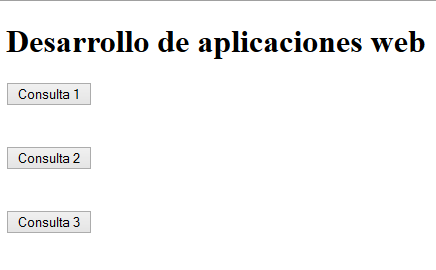
\includegraphics[scale=0.5]{imagenes/inicio.png}
	\end{center}
	\caption{Figura de la interfáz de inicio de la página web de consultas.}
\end{figure}
 
 

\bibliographystyle{plain}
\bibliography{informe,terminologia}

\end{document} 